\documentclass[a4paper]{article} 
\usepackage[dutch]{babel}
\usepackage{graphicx}
\usepackage{color}
\usepackage[final]{pdfpages}
\usepackage{hyperref}

\usepackage[margin=2.9cm]{geometry} %ik denk dat de we wel een redelijk aantal paginas gaan hebben wanneer het verslag klaar is, de standaardmarges van latex zijn echt wel groot
%\usepackage[utf8x]{inputenc} uitgeschakelt aangezien ik dit package niet heb, gebruik escape codes of hercompile de pdf zelf om speciale tekens te gebruiken


\title{SWOP - Hospitaal Iteratie 3}
\author{Groep12\\ \\Jeroen Van Gool\\Ruben Lapauw\\Tom De Bie\\Jeroen De Coninck}
\date{}
\pdfinfo{
	/Title (SWOP - Hospitaal Iteratie 3)
	/Author	(Groep\ 12)
}

\begin{document}
\maketitle
\newpage
\tableofcontents
\newpage

\section{Inleiding}
\subsection{Overzicht van het verslag}
In dit verslag bespreken we het design van een uitgebreid software-systeem ontworpen voor het management van een hospitaal. Het systeem biedt momenteel ondersteuning voor een verscheidenheid aan gebruikers, zijnde dokters, verpleegsters, magazijnbeheerders en de hospitaalbeheerder. Pati\"enten kunnen geregistreed worden in het systeem waarna er diagnoses, medische testen en behandelingen voor hun aangemaakt kunnen worden. Verder biedt het systeem ook mogelijkheden voor het beheer van machines in het hospitaal een het plannen van afspraken tussen hospitaalpersoneel, machines en patienten.

In deel 2 van het verslag, 'Het systeem', geeft men eerst een klein overzicht van ons Hospitaal-systeem. Daarna wordt er \'e\'en voor \'e\'en op elk subsysteem gefocust.
Voor elk subsysteem begint men eerst met een beschijving van het systeem, waarna men volgt met de bespreking van een relevante use case, waarmee men het gebruik van het systeem illustreert.

Deel 4 bevat een conclusie met een reflectie over de sterke en zwakke punten van de implementatie. Tenslotte in deel 5 zijn alle appendices verzameld, deze bevatten informatie die in het verslag hoort, maar het ge\"implementeerde basissysteem niet bespreken (met uitzondering van het volledige klassendiagram natuurlijk).
\subsection{Veronderstellingen \label{sec:assumptions}}
\begin{itemize}
\item ''Een pati\"ent kan aan niet meer dan 10 X-ray scans per jaar onderworpen worden.'' 
Hierbij hebben we natuurlijk aangenomen dat het over de tijdspanne van een jaar gaat, 
en niet over een kalenderjaar.
Dit is natuurlijk gemakkelijk aanpasbaar.
\item Personeelsleden alsook pati\"enten hebben een unieke naam. 
Je kan echter wel een pati\"ent hebben met dezelfde naam als iemand van het personeel, 
dit leek ons logisch aangezien een personeelslid ook opgenomen kan worden in het ziekenhuis als hij of zij zelf ziek is.
\item De FIFO-queue wordt nu gebruikt zoals gevraagd. Dit was geen probleem met de implementatie.
\item Bij het doorspoelen van de tijd wordt als het eten op is geen eten meer gegeven aan de pati\"enten.
\item De Stock van alle items is voldoende groot dat er niet meer items gevraagd worden dan dat het minste aantal items die in een Stock kan ziten zonder dat er bijbesteld moet worden. Met andere woorden, deze is voldoende groot dat  2 dagen na de laatste afspraak altijd voldoende items zullen zijn.
\item Als de tijd doorgespoeld wordt, wordt er gevraagd om medical tests en treatments tot op de vorige dag in te vullen. We gaan niet tot de dag zelf om de nurses ook nog een kans te geven resultaten in te vullen.
\end{itemize}
\section{Het systeem}
\subsection{Overzicht} %Informatie in het systeem.???
Het hospitaal heeft verschillende subsystemen: 
De wereld die als oer-Object dient. 
Deze houdt de tijd, personen, machines en campussen bij, de campussen houden elk hun eigen voorraden bij.
De personen splitsen zich op in pati\"enten en personeel. 
Het personeel kan verschillende operaties uitvoeren op het systeem, 
waarvan de volgende op pati\"enten toegepast worden: 
voeg diagnoses, medische testen en behandelingen toe. 
Medische testen en behandelingen hebben beiden een afspraak die als alle andere precondities voldaan zijn aangemaakt worden. 
Verder is er ook voorraad; deze voorziet maaltijden voor de pati\"enten en andere items voor de behandelingen. 
De bestellingen gebeuren hiervan automatisch. Aangekomen bestellingen worden niet automatisch verwerkt.


\subsection{Gebruikers \label{sec:users}}
\subsubsection{Beschrijving}
Het login-subsysteem is gecentreerd rond het concept van ''LoginControllers''. Een LoginController in ons Hospitaal-systeem is een object dat een gebruiker representeert voor de duratie dat deze gebruiker aangemeld is, het object wordt dus ge\"invalideerd zodra de gebruiker zich afmeldt.
Naast de huidige gebruiker te identificeren in verscheidene functies biedt een LoginController ook methoden aan om informatie op te vragen over de gebruiker of om bepaalde acties uit te voeren op informatie waartoe het gebruikers-object toegang heeft.

De klasse LoginController wordt zelf nooit ge\"instantieerd: enkel subklassen worden gebruikt. Deze subklassen zijn elk gespecialiseerd in een bepaalde rol in het ziekenhuis, zo zijn er bijvoorbeeld DoctorControllers en NurseControllers die functionaliteit aanbieden specifiek aan respectievelijk dokters en verpleegsters. Natuurlijk zijn er ook LoginControllers voor elke andere personeelsrol in het hospitaal.

Het grote voordeel van deze organisatie van LoginControllers is dat we deze objecten nu ook kunnen gebruiken om ervoor te zorgen dat bepaalde acties enkel uitgevoerd worden door bevoegd personeel. Door bij deze acties een specifieke subklasse van LoginController te eisen kan dit verzekerd worden. Een geldige LoginController voor een bepaalde rol kan namelijk enkel verkregen worden via de correcte uitvoering van de aanmeld-procedure.
\subsubsection{Usecases: Login, Logout}
De gebruikers (het personeel) kunnen zich aanmelden op het systeem, bij het aanmelden kunnen ze kiezen op welke campus ze aanwezig zijn. 
Dit gebeurt aan de hand van een lijst van CampusInfo-objecten die via een WorldController opgevraagd worden aan de World. 
CampusInfo is een object dat enkel de informatie bevat die nodig is om een Campus te identificeren (in dit geval de naam).
Met dit identificatie-object kan de \texttt{login}-methode van de WorldController de juiste campus opvragen om een CampusController voor te maken.
Deze CampusController wordt doorgegeven voor gebruik door LoginControllers, zoals bv. de DoctorController of de NurseController.
Na dat de gebruiker klaar is met het systeem kan men de gebruiker eenvoudig afmelden door de methode \texttt{logout()} van het LoginController-object aan te roepen. Deze invalideert het object waardoor het niet meer gebruikt kan worden.

Om het gebruik van deze LoginControllers te illustreren zullen we de procedure voor het aanmelden eens dichter bekijken (zie figuur~\ref{fig:login}).
Indien we het systeem als black box bekijken zien we dat we slechts twee API-calls nodig hebben om zich aan te melden, de eerste om een lijst van alle gebruikers in het systeem te krijgen (een LoginInfo bevat alle informatie om een gebruiker te identificeren in het systeem: de naam en de rol), de tweede voor het echte aanmelden en daarmee ook het verkrijgen van een LoginController-object. In het getoonde system sequence diagram is nog de extra stap getoond waarin de user interface de rol van de gebruiker opvraagt en daarop gebaseerd het juiste menu kiest om te tonen, meer over de UI is de vinden bij de appendices, in sectie~\ref{sec:ui}.
\begin{figure}[h]
\centering
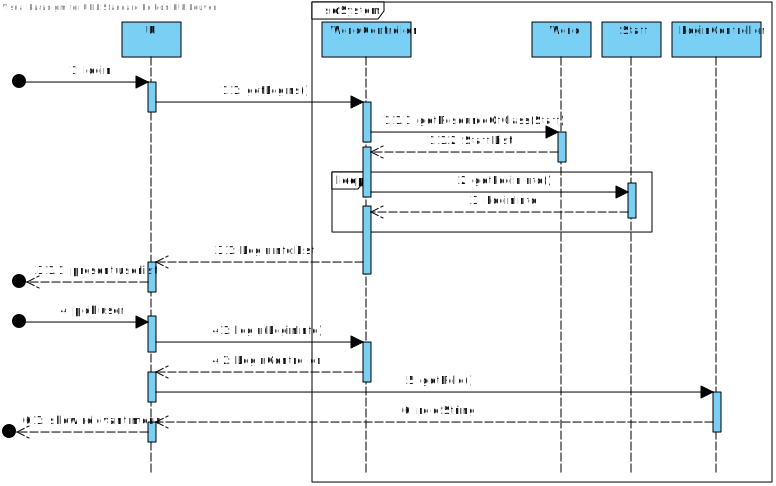
\includegraphics[width=\textwidth]{Pictures/Login}
\caption{Use-case: Login}
\label{fig:login}
\end{figure}

Nu dat we een LoginController hebben kunnen we deze meegeven aan andere controllers die onze LoginController vervolgens kunnen gebruiken voor acties die een gebruiker in een bepaalde rol nodig hebben; bijvoorbeeld een MedicalTestController die een DoctorController vereist om medische testen te kunnen plannen.

\subsubsection{Bespreking GRASP, uitbreidbaarheid en nadelen}
Door de personen geabstraheerd als Schedulable bij te houden in de wereld verliest deze een hele hoop koppelingen met de personen. Er moet nu wel iedere keer gefilterd worden op klasse om een groep personen op te vragen van een bepaald type. Het voordeel is nu wel dat men een heel flexibele methode heeft om de personen te filteren: men kan bijvoorbeeld alle Personeelsleden filteren door Staff.class te gebruiken. Als men verschillende klasses opvraagt en dan de lijsten merged kan men elke combinatie van groepen maken, zonder dat de wereld moet veranderen. Deze lage koppeling zorgt voor een uitbreidbaar design, er kunnen gemakkelijk nieuwe types toegevoegd worden zoals de Warehousemanager.
Het gebruik van de CampusInfo-objecten zorgt ervoor dat de gebruiker van de API nooit een echt Campus-object te zien krijgt, een hele hoop koppeling is dus vermeden hierdoor. Verder zorgt deze aanpak ervoor dat er geen onge\"oorloofde toegang tot de Capmus-objecten is.

Er kunnen geen meerdere verantwoordelijkheden gelegd worden bij de verschillende personen: een HospitalAdministrator kan geen docter of pati\"ent zijn. Hiervoor zou het design moeten aangepast worden naar een decoratorpatroon.


\subsection{Input en output}
\subsubsection{Beschrijving}
Input en output is is strikt gereguleerd. Alle output moet ofwel immutable zijn, zoals Strings en andere, ofwel read-only, zoals CampusInfo en LoginInfo, ... 
Voor Input moet men ook oppassen: deze moet ook immutable zijn, ofwel moet men een perfecte kopie maken van alle Objecten die ingegeven worden. Maar alleen met primitieven en Strings werken is niet uitbreidbaar en onhandig werken.
Men kan bijvoorbeeld niet garanderen dat alle behandelingen hetzelfde aantal parameters hebben van hetzelfde type. 
De oplossing is om de parameters te abstraheren naar een Argument-object. 
Om de kennis van in het systeem dan ook nog af te schermen van de UI is er een vraag bij deze objecten gegeven. Hierdoor moet de UI niet de vragen stellen aan de gebruiker en kunnen gemakkelijk nieuwe behandelingen met andere parameters toegevoegd worden. Een ander gevolg is dat men direct kan controleren of de invoer mogelijk correct is.

\subsubsection{Publieke Werking}
De interface PublicArgument<E> is de basis van de invoer. Deze heeft een vraag die aan de gebruiker moet gevraagd worden en deze kan beantwoord worden door de \texttt{setAnswer}-methode met een String. Deze wordt direct geconverteerd naar het type E. Deze Argumenten zitten in een ArgumentList, samen met objecten van de superklasse Argument<E>. Deze Argument<E>-objecten zijn voor het interne systeem om in te vullen, op het moment dat de UI de controle teruggeeft aan het systeem.  

\subsubsection{Interne Werking}
Een generische factory verwacht als invoer om een nieuw object te maken een lijst van Arguments. Men kan een nieuwe lege lijst van Argumenten opvragen aan deze factory met de methode \texttt{getEmptyArgumentList}. Als deze ingevuld is door de UI en door de andere code kan met de \texttt{validate}-methode gecontroleerd worden of een lijst correct is voor een bepaalde factory zonder deze factory een object te laten maken. Bij het aanroepen van de \texttt{make}-methode aangeroepen met deze lijst om een object aan te maken zal eerst automatisch deze \texttt{validate} aangeroepen worden om te controleren of de invoer wel geldig is.

\subsubsection{Bespreking GRASP en uitbreidbaarheid}
Deze opbouw laat toe om een grote diversiteit aan invoer uit te lezen op een veilige en generische manier. Het laat toe om de input statisch te valideren tijdens de invoer en zo duidelijker fouten terug te geven wat de cohesie ten goede komt. Het laat ook toe om informatie van het systeem te lezen zonder dat de UI deze zelf moet zoeken. Hierdoor is de koppeling tussen de UI en het systeem lager en duidelijk herkenbaar. 

Men kan eenvoudig nieuwe argumenten ontwerpen en gebruiken zonder dat er iets moet veranderen aan de UI. Om informatie van andere objecten mee te geven kan men gebruik maken van het visitor-pattern en een filter.

\subsection{Diagnoses \label{sec:diagnosis}}
\subsubsection{Beschrijving}
Functionaliteit omtrent diagnoses wordt voorzien door de DiagnosisController. Interactie via dit object zorgt ervoor dat de gebruiker van de API geen weet hoeft te hebben van de interne werking van het systeem. De enige diagnose-gerelateerde functie voor eindgebruikers die niet door de DiagnoseController afgehandeld wordt zijn de \texttt{getSecondOpinions} en de \texttt{removeSecondOpinion} methoden in de DoctorController (een type LoginController, zie sectie~\ref{sec:users}), aangezien deze enkel gebruik maken van informatie in het DoctorController-object. Deze methoden komen verderop nog aan bod.

Een DiagnosisController krijgt bij constructie een geldige DoctorController en WorldController mee: deze functionaliteit is dus enkel beschikbaar voor aangemelde dokters. De WorldController geeft gecontroleerde toegang tot de benodigde andere objecten en subsystemen in de wereld.
De DiagnosisController werkt met Diagnosis-objecten (en bijgevolg ook DiagnosisSecondOpinion-objecten voor diagnoses die door een andere dokter nagekeken moeten worden, deze zijn een subklasse van Diagnosis). Deze worden  via de methode \texttt{enterDiagnosis} aangemaakt in de DiagnosisFactory-objecten die bestaan in de wereld.

Deze diagnoses worden bijgehouden in de patient (de patientfile is een view op een patient) waarvoor de diagnose gemaakt is, en indien een controle door een andere dokter vereist is, bij het Doctor-object van de dokter die de diagnose moet nakijken.
Een diagnose kan een bijhorende Treatment bijhouden (meer informatie over Treatments is te vinden in sectie~\ref{sec:treatment}), in het geval van een DiagnosisSecondOpinion wordt deze automatisch gepland zodra de diagnose goedgekeurd wordt.

Om het ongedaan maken van acties te ondersteunen wordt elke actie via een Command-object uitgevoerd dat bij de uitvoerende dokter bijgehouden wordt. Hierop kan eenvoudigweg \texttt{undo} aangeroepen worden om een actie ongedaan te maken.
\subsubsection{Usecases: EnterDiagnosis, ApproveDiagnosis}
\begin{figure}[h]
\centering
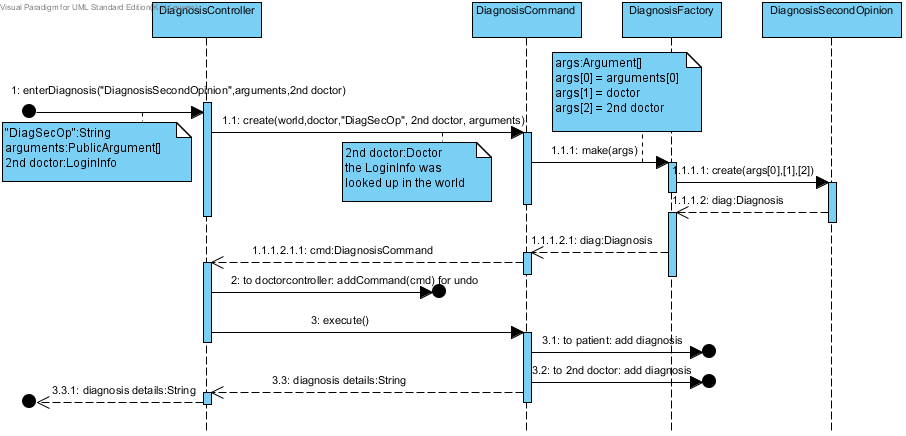
\includegraphics[width=\textwidth]{Pictures/EnterDiagnosis}
\caption{Interne verwerking van een \texttt{enterDiagnosis}-aanroep}
\label{fig:enterdiagnosis}
\end{figure}

In figuur~\ref{fig:enterdiagnosis} zien we hoe een gegegeven DiagnosisController-object een \texttt{enterDiagnosis}-aanroep verwerkt voor diagnose met second opinion. Bij normaal gebruik wordt deze aanroep voor gegaan door aanroepen naar \texttt{getAvailableDiagnosisFactories}, \texttt{getDiagnosisArguments} en \texttt{getAvailableSecondOpinionDoctors} om correcte waarden te bekomen voor de respectieve parameters. Indien ongeldige waarden gebruikt worden zal het systeem een gepaste exception geven. De naar rechts wijzende lost messages duiden op plaatsen waar verwijzingen naar het Diagnosis-object (of het geval van \texttt{addCommand} het Command-object dat de diagnose heeft aangemaakt) worden bijgehouden.
\begin{figure}[h]
\centering
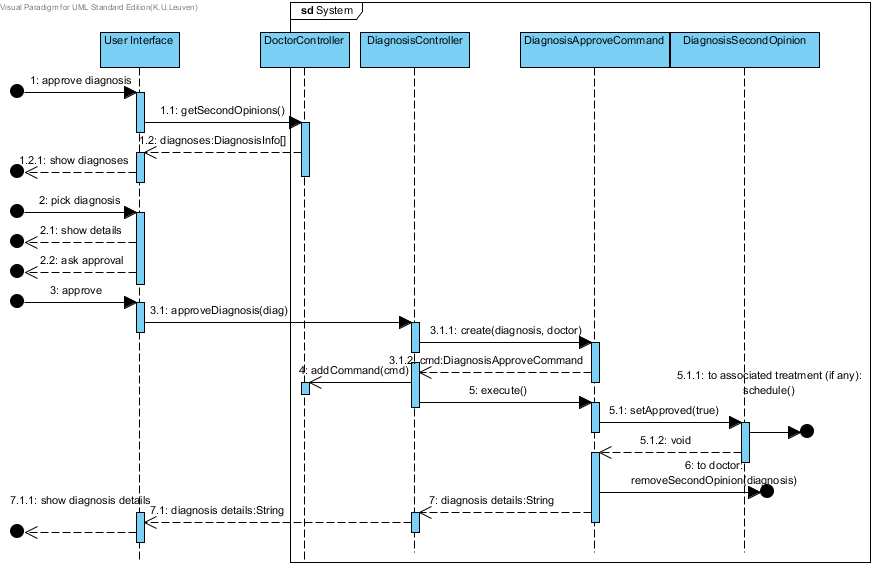
\includegraphics[width=\textwidth]{Pictures/ApproveDiagnosis}
\caption{Use-case: Approve diagnosis}
\label{fig:approvediagnosis}
\end{figure}
Om een diagnose goed te keuren (zie figuur~\ref{fig:approvediagnosis}) zal het systeem een ApproveDiagnosisCommand-object aanmaken dat, wanneer uitgevoerd, de diagnose als geldig markeert en de diagnose verwijdert uit de lijst van diagnoses die nog gecontroleerd moeten worden. De diagnose zal daarop de bijhorende behandeling (indien deze bestaat) plannen. Meer informatie over behandelingen en tijdsplanning kan gevonden worden in secties~\ref{sec:treatment} en \ref{sec:scheduling}.

In het geval dat de dokter de diagnose afkeurt zal het systeem eenvoudigweg de diagnose verwijderen uit de lijst te controleren diagnoses en een nieuwe DiagnosisWithSecondOpinion aanmaken waarbij de dokter waarvan de mening gevraagd moet worden automatisch ingevuld wordt als de dokter die de originele diagnose gemaakt heeft.
\subsubsection{Bespreking GRASP}
De koppeling is zo laag mogelijk gehouden door de verschillende diagnoses met een gemeenschappelijke superklasse te hebben. Deze voorziet de basistoegang tot alle diagnoses. Ook de verschillende soorten treatment zijn geabstraheerd, wat een logische stap is. Door de verbindingen enkel in een enkele richting te hebben wordt de koppeling nog verder verminderd: een diagnose weet niet tot welke patient behoort. Een doctor weet niet welke diagnoses hij allemaal gemaakt heeft... 

De cohesie is ook groot, vooral in termen van de informationexpert, de informatie over diagnoses worden in de objecten zelf bijgehouden en is netjes afgeschermd van de rest van het systeem. Enkel de koppelingen, die laag zijn, kunnen de diagnose veranderen.

Aangezien er niet echt een duidelijke uitbreiding beschikbaar was om het design te controleren kunnen er een aantal probleemgevallen voorkomen. Een eerste aanpassing zal waarschijnlijk de abstractie van een diagnose naar een interface zijn. Nu was door de simpele uitbreiding het voldoende een uitbreidende klasse te maken. Het gebruik van de Command en de Factory met argumenten zou nog steeds flexibel genoeg moeten zijn.


\subsection{Magazijn}
\subsubsection{Beschrijving}
Hier volgt een overzicht van de belangrijkste klassen en een korte beschrijving van hun taken in ons ontwerp van het magazijn systeem:
\begin{itemize}
\item Stock :  Deze klasse is verantwoordelijk voor het bijhouden van de voorraad van 1 soort item. De klasse Stock voorziet methodes om items te reserveren en te verwijderen uit de voorraad.
\item Warehouse : Deze klasse bevat verschillende instanties van de klasse Stock, meer bepaald voor ieder soort item in het systeem één Stock. Deze klasse heeft methodes om de juiste stock te verkrijgen en om orders toe te voegen aan de bijhoorde stock.
\item Items: De verschillende klassen in het package Items stellen de concrete items voor. Deze klassen zijn subklasse van de klasse Item. In deze klasse wordt bijgehouden of een item gereserveerd is en de vervaldatum van het item.
\item OrderList: De klasse Stock bevat een OrderList. Deze Orderlist is verantwoordelijk voor het bijhouden van de verschillende bestellingen voor de Stock.
Order: Deze klasse stelt een bestelling voor en bevat de informatie van deze bestelling.
\item OrderPlacers: De klassen in dit package zijn verantwoordelijk voor te bepalen wanneer er moet worden bijbesteld.
\item LIFO-queue: Dit is een FIFO-queue geworden zoals voorzien.
\item FIFO-queue: Een wrapper rond Queue<E> en geabstraheerd als ItemQueue.
\item ItemReservator: Deze klasse is verwijderd. En is vervangen door de ItemReservationCommand. Deze heeft een andere naam en andere verantwoordelijkheden.
\item ReserveItemObserver: Deze klasse is verwijderd, een afspraak wordt direct gepland op het moment dat alle items beschikbaar zijn.
\item ItemReservationCommand: Deze klasse reserveert alle nodige items in een stock. Op het moment van de afspraak komen de Items in deze klasse beschikbaar.
\item ItemInfo: Dit object is een veilig object om buiten het systeem te gebruiken. 
\item ItemConstraint: Deze constraint wordt bij het maken van een afspraak in rekening gebracht om een goed moment van afspraak te vinden.
\end{itemize}

\subsubsection{Interne Werking}
In tegenstelling tot een eerdere implementatie waar afspaken pas gepland werden als we zeker waren dat alle items op voorrad waren, wordt een afspraak nu wel direct gepland. Een geschiedenis van alle afspraken wordt voor ieder type item bijgehouden en bij het plannen van de afspraak wordt een moment gezocht waar  er geen tekort aan items is, noch waar er ooit in de toekomst problemen zullen komen. Het gebruik van een Item kan zich ver in de toekomst propageren en zo binnen een aantal maanden een probleem veroorzaken. 
\subsubsection{Bespreking GRASP}
De warehouse is weer gemaakt om een zo laag mogelijke koppeling te hebben. De warehouse weet niet aan welke campus hij verbonden is, hij verzameld enkel alle verschillende stocks. De stocks weten ook niet tot welke wereld ze behoren. Dit zorgt voor een strikte afscheiding tussen de objecten en hun informatie. De lijst van orders is ook enkel gekend door de stock en bepaald welke items er besteld zijn. Het gebruik van een stockobserver verminderd ook de koppeling in stock sterk.

De twee subsystemen, het Warehouse en de Scheduler, zijn enkel met een Constraint (zie tijdsplanning, sectie \ref{sec:scheduling} verbonden. Dit garandeerd een minimale koppeling. De constraint zelf bevat ook weinig logica en wordt door een afgescheiden algoritme afgehandeld dat apart getest kan worden.
\subsubsection{Nadelen}
Bij het plannen wordt geen rekening gehouden met het eventuele vervallen van de items aangezien we dit niet kunnen voorspellen. Het gebruik van een FIFO-queue en een ``druk'' hospitaal zorgen ervoor dat deze kans klein is. 

\subsection{Medische testen en behandelingen \label{sec:medicaltest} \label{sec:treatment}}
\subsubsection{Beschrijving: medische testen}
De abstracte klasse MedicalTest implementeert de interface Result omdat het resultaat moet kunnen worden toegevoegd aan en opgevraagd uit de MedicalTest. Een MedicalTest implementeert ook de interface Appointable, omdat een MedicalTest een reden is om een afspraak te maken. In het systeem bestaan er op dit moment 3 verschillende subklassen van MedicalTests, namelijk XRayScan, UltraSoundScan en BloodAnalysis. Bij creatie van zo'n subklasse worden de parameters gecontroleerd en indien nodig wordt er een ArgumentConstraintException gegooid. Zo zal de UI een error kunnen melden indien er bijvoorbeeld een XRayScan met zoom 5 gemaakt zou worden. 

Wegens het gebruik van preemptive-scheduling zal het plannen van een medische test voornamelijk besproken worden in de sectie Scheduling\ref{sec:scheduling} worden uitgelegd. De prioriteit van deze Appointment wordt gevraagd via een PriorityArgument.

\subsubsection{Beschrijving: behandelingen}
De abstracte klasse Treatment implementeert ook de interfaces Result en Appointable, om dezelfde redenen als een MedicalTest. In het systeem zijn er op dit moment 3 subklassen, namelijk Cast, Medication en Surgery. Bij het aanmaken van zo'n subklasse worden ook hier de paramenters gechecked en indien nodig wordt er een ArgumentContraintException gegooid.

Elke subklasse heeft opnieuw een Factory, die bij creatie van de wereld in de wereld wordt aangemaakt. De TreatmentController en TreatmentResultController zorgen voor interactie tussen de UI en het systeem op gebied van Treatments. Ook het plannen van een treatment komt wordt wegens het gebruik van preemptive-scheduling verduidelijkt in de sectie Scheduling\ref{sec:scheduling}.

\subsubsection{Verloop usecases: OrderMedicalTest en EnterTreatment}
Bij het cre\"eren van een MedicalTest, wordt er een MedicalTestCommand gemaakt die op zijn beurt een MedicalTest laat aanmaken door de juiste MedicalTestFactory. Vervolgens maakt de MedicalTestCommand ook een AppointmentCommand aan voor het schedulen van de MedicalTest. Daarna voegt de MedicalTestController het Command toe aan de DoctorController. Vervolgens wordt het command uitgevoerd, de MedicalTest wordt toegevoegd aan de Patient. Ook wordt de test gescheduled: AppointmentCommand wordt uitgevoerd.
\begin{figure}[h]
\centering
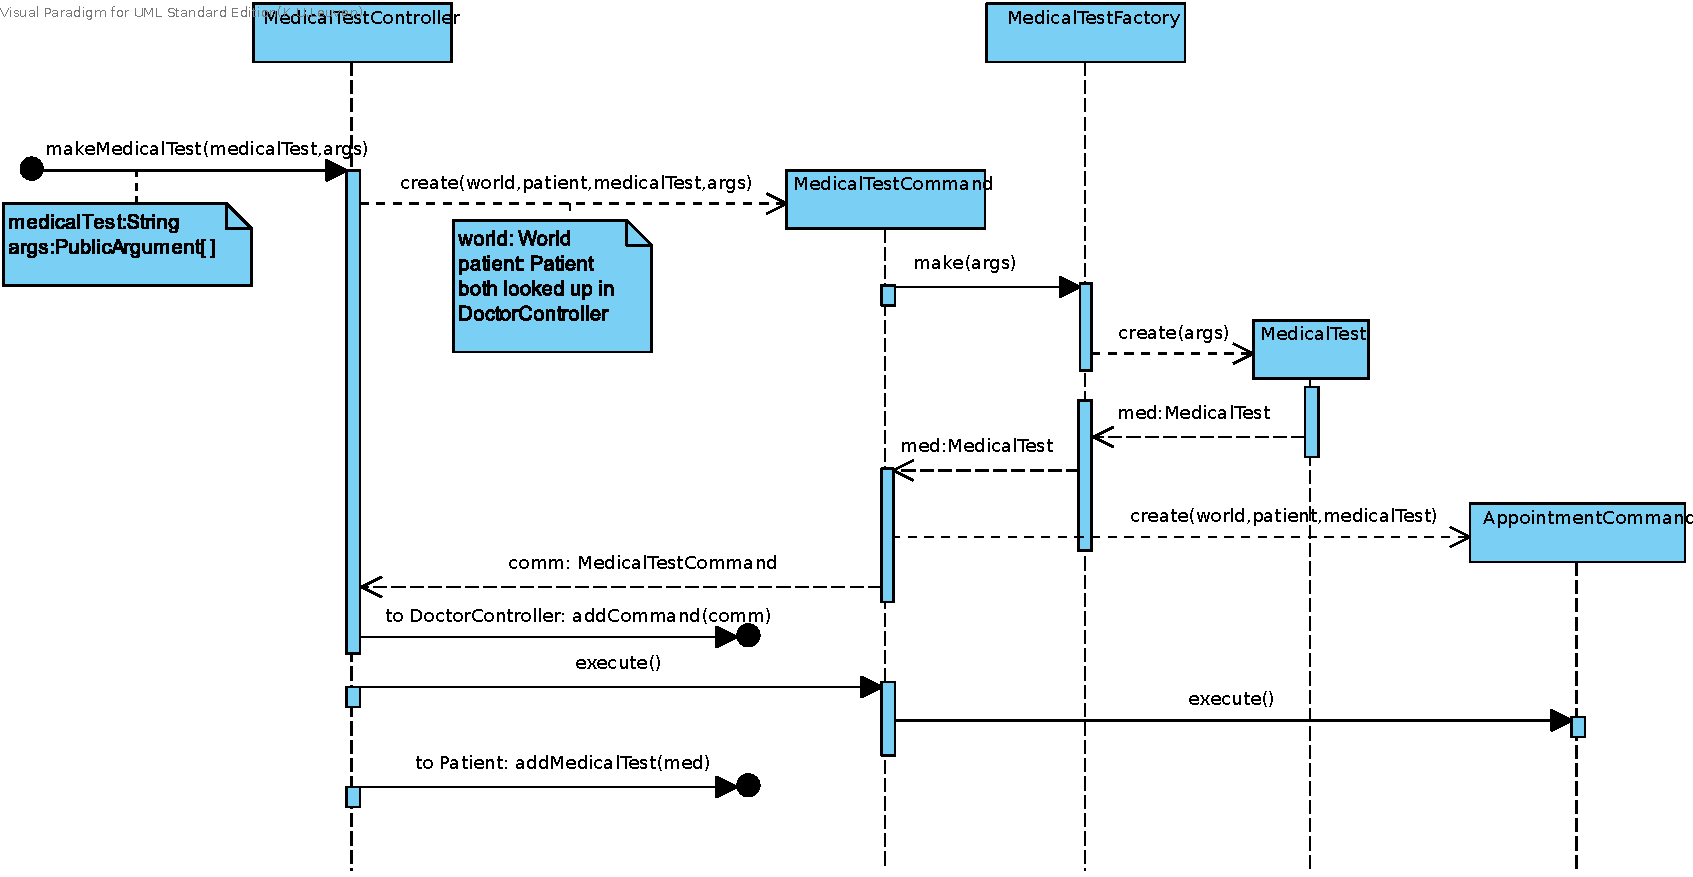
\includegraphics[width=\textwidth]{Pictures/OrderMedicalTest.pdf}
\caption{Use-case: Order medical test}
\label{fig:ordermedicaltest}
\end{figure}
Het maken van een behandeling gebeurt analoog.
\subsubsection{Bespreking GRASP en uitbreidbaarheid}
De verschillende types medische testen en behandelingen zijn heel uitbreidbaar. Er kunnen gemakkelijk andere behandelingen toegevoegd worden: Je maakt een nieuwe behandeling en zijn bijhorende factory. Het enige probleem is dat de nieuwe types misschien informatie van binnen het systeem nodig hebben, zoals diagnoses met een second opinion. In dat geval zou men een visitorpatroon moeten gebruiken om de argumenten te beantwoorden. De uitbreidbaarheid is getest geweest door maar één medische test en één behandeling te implementeren zoals gezegd in teststrategy report. Dit werkte zonder problemen: alle domein informatie moest eenvoudigweg geïmplementeerd worden. 

De cohesie wordt sterk verhoogt door de creatie af te scheiden van het effectieve object door een factory te gebruiken. Dit zorgt ook direct dat wereld geen enkele connectie moet hebben met de behandelingen zelf, alleen met objecten die ze maken. Door dit verder te abstraheren daalt de koppeling nog verder. Het gebruik van een command schermt het volledige subsysteem af door een facade. Dit verlaagt de koppeling met externe klassen.

\subsection{Tijdsplanning \label{sec:scheduling}}
\subsubsection{Beschrijving}
Het maken van een afspraak is een complex systeem. Het gebruik van AppointmentCommand laat toe om acties ongedaan te maken en te herdoen zonder alle informatie terug op te vragen. Dit houdt wel in dat het rekening moet houden met de veranderingen van het systeem. De ScheduleGroups laten toe om dit op een manier te doen zonder dat de command moet aangepast worden, andere flexibiliteit is dat er andere soorten groepen ook kunnen toegevoegd worden met dezelfde API. Ook het selecteren van ScheduleGroups van zowel binnen het systeem (treatment.getScheduleGroups) als buiten het systeem laten een grote flexibiliteit. Een stagair die aanwezig moet zijn op een bepaalde Surgery kan eventueel op de volgende manier toegevoegd worden: maak de afspraak ongedaan, voel een ScheduleGroup van de stagair bij en doe deze opnieuw. Hiervoor moeten enkel methoden om de afspraak op te vragen en om de stagair toe te voegen bijgemaakt worden. 

Het gebruik van constraints op de groepen laat ook een grote vrijheid over. Doordat deze met een visitorpatroon werkt kan deze een hele hoop Schedulable overweg met kleine aanpassingen. Zo is de XRayConstraint voor Patient en de constraint op de werkuren voor Nurses. De TimeDelay is ook aanpasbaar een mogelijke uitbreiding is bijvoorbeeld een vertraging tot na een bepaalde datum. Dit kan gewoon door de getDelayedTimeFrame en setWorld in een interface te gieten.

Afspraken worden gemaakt voor een Appointable, dit wordt gedaan door AppointmentFactory. Deze krijgt toegang tot een aantal Constraint-objecten; deze kunnen pas valideren als aan de voorwaarde die ze opleggen (bv. niets schedulen buiten de werkuren). De AppointmentFactory zoekt een moment waarop alle constraints voldaan zijn. Ook is de eerste constraint een GetCampusConstraint voor ieder type van afspraak: deze bepaalt de campus waarop de afspraak zich zal voordoen.

Voor een afspraak tussen een dokter en een pati\"ent moeten bijvoorbeeld aan volgende Constraints voldaan zijn: 
DoctorBackToBackConstraint (DoctorPatientAppointment), Preference (van Doctor), PriorityConstraint (DoctorPatientAppointment),  en WorkingHoursConstraint (Doctor). 
Elk van deze constraints maken deel uit van alle voorwaarden die opgelegd zijn aan de afspraken. 
De PriorityConstraint zorgt dat er geen twee appointments op hetzelfde moment vallen en als er op een afspraak op dat moment staat bij een persoon dat die een lagere prioriteit heeft en dus zal verzet worden. De DoctorBackToBackConstraint zorgt ervoor dat de afspraak ofwel op het uur valt ofwel dat de afspraak direct na de vorige valt.

\subsubsection{Bespreking GRASP en uitbreidbaarheid}
Door de abstractie van behandelingen, die een soort afspraken zijn, en het effectieve afspraak-object door een interface is het subsysteem veel losser gekoppeld aan de Appointables.
Dit zorgt ook voor een grotere cohesie: de informatie zit afgeschermd in een eigen object met een zeer specifiek doel. Het gebruik van een command laat toe om vaak gebruikte code te hergebruiken. Hierdoor ontstaat er een lagere koppeling in TreatmentCommand met het subsysteem en is er hogere cohesie: de code van een behandeling bij TreatmentCommand en de afspraak bij AppointmentCommand.

De code zelf heeft weinig uitbreiding nodig. Een afspraak is altijd hetzelfde formaat. De groepen zijn ook heel finaal, je zou misschien een groep kunnen toevoegen met één van de volgende vaste schedulables, maar dan zou je alle mogelijke groepen moeten hebben.

Ook de koppeling tussen de twee belangrijkste systemen is hier laag: De scheduler weet niet eens of er iets in het warehouse gedaan wordt. En behalve dat het opvragen van alle benodigde informatie is alles afgeschermd. De scheduler weet enkel dat hij constraints opvraagt van een Schedulable, en van een Appointable.
De constraints hangen in een ketting: elk Constraint heeft de kans om een gekozen tijd en plaats af te wijzen, indien niet geeft hij de verantwoordelijkheid van het afwijzen door aan het volgende Constraint-object. Hierdoor kan men zeer eenvoudig meer constraints toevoegen of weghalen, men hoeft enkel de ketting langer te maken, of in te korten met de juiste Constraints zoals het nodig is.

Het algoritme is ook afgeschermd in een eigen deel binnen dit systeem. Dit laat toe om snellere algoritmes te gebruiken, zoals constraintprocessing met backjumping, ...

\subsection{Administratie}
\subsubsection{Beschrijving}
Administration gebeurt aan de hand van het aanroepen van Controllers die op hun beurt de Wereld gaan updaten. Zo zijn er de StaffController die Staff kan toevoegen, de MachineController die Machines kan toevoegen en de AdministratorController die alles afhandelt ivm het vooruitgaan van de tijd.
\subsubsection{Verloop usecase: Add staff \& machine}
Eerst vraagt de AddStaffUI alle StaffFactories op van de StaffController en laat hij de gebruiker kiezen tussen deze Factories. Vervolgens vraagt hij de arguments op die ingevuld moeten worden. En ten slotte laat de StaffController de Factory de Staffmember aanmaken en stopt hij deze weg in de recources van de World. Indien er reeds Staff bestaat met de ingegeven naam, dan zal er een foutmelding worden meegedeeld.
Om machines toe te voegen volgt men een analoge procedure aan die voor het toevoegen van een personeelslid.
De meest recente toevoeging aan het systeem is het gebruik van campussen. Indien een personeelslid of een machine met een vaste plaats aangemaakt wordt, zal er vanaf heden dan ook gevraagd worden op welke campus deze zich bevinden.

\section{Onbresproken Usecases}
\subsection{Preference}
Deze usecase is eenvoudig. Een ListArgument van alle beschrijvingen van preferences worden opgevraagd en dan deze set dan de preference van de doctor. De PreferenceConstraint vraagt deze op en controleert alle mogelijke momenten met deze preference. Om een nieuwe preference te maken moet men een klasse maken die de interface Preference uitbreidt.

\subsection{Undo \& Redo}
Iedere operatie kan in een Command gewrapped worden. Dit zorgt voor de mogelijkheid om een operatie uit te stellen en indien mogelijk ongedaan te maken en herdaan worden. Deze abstractie laat ook toe om deze operaties bij te houden om ongedaan te maken. De gedane Commands worden bijgehouden in een lijst bij de doctorcontroller: de operaties zelf maken geen deel uit van het systeem. Het gevolg is dat bij het uitloggen alle gedane operaties permanent uitgevoerd worden. Indien dit wel nodig is, kunnen de twee lijsten in de doctor zelf bijgehouden worden en dus persistent gemaakt worden.

\subsection{Consult Patientfile}
De open Patientfile usecase vraagt eerst alle PatientInfo objecten aan de WorldController via de DoctorController om deze dan te gebruiken om een Patient in te laden bij de Doctor.

\subsection{Close Patientfile}
Deze usecase zet de PatientFile op null bij de doctor.

\subsection{Discharge Patient}
Een dokter kan een pati\"ent ontslaan door simpelweg de methode \texttt{dischargePatient} van zijn DoctorController aan te roepen. Dit heeft als gevolg er aan het openstaande Patient-object gevraagd wordt of deze pati\"ent onstlaan kan worden. Het Patient-object controleert in zijn gegevens of nog onbehandelde diagnoses zijn of medische tests/behandelingen zonder resultaat, indien dit niet het geval is kan de pati\"ent ontslaan worden.
De pati\"ent wordt zodanig gemarkeerd en alle pati\"ent-gerelateerde functies en methoden in de DoctorController zullen een fout genereren tot een nieuwe pati\"ent geopend wordt.
\subsection{Register Patient}
Om een bestaande pati\"ent op te nemen hoeft een aangemelde Nurse (die bijgevolgd toegang heeft tot een NurseController) enkel aan de wereld vragen achter de lijsten van patienten en dokters in het systeem. Uit deze lijsten kunnen dan de gepaste argumenten gekozen worden voor de /texttt{checkIn}-functie van de NurseController. Dit heeft als resultaat dat de pati\"ent als opgenomen geregistreerd wordt en er meteen ook een afspraak met de gegeven dokter gepland wordt (voor details over tijdsplanning zie sectie~\ref{sec:scheduling}).

Indien de pati\"ent nog niet geregistreerd is in het systeem zal dit eerst gedaan worden volgens het Factory-systeem dat doorheen heel het project  gebruikt is. Nadat de pati\"ent geregistreerd is kan men verder zoals beschreven in de eerste paragraaf.
\subsection{Enter Medicaltest result}
EnterResult wordt opgeroepen met argumenten: MedicalTestInfo en args (in te vullen testresults). Hierop gaat de MedicalTestController zoeken tussen alle medicaltesten van alle pati\"enten, welke ingevuld moet worden. Ten slotte worden de results toegevoegd. Indien er foute argumenten worden meegegeven, dan zal de gepaste foutmelding worden weergegeven.

\subsection{Enter TreatmentResult}
Door het gebruik van een geschiedenis in het Warehouse kunnen resultaten pas ingevuld worden wanneer de items er uit verwijderd zijn. En dit mag enkel op het juiste moment, anders kan zal de planning niet meer juist werken. Het is dus logisch dat resultaten pas uitgevoerd kunnen worden als het na de start van deze afspraak is. Anderzijds moet men tijdens het vooruitspoelen van de tijd direct de resultaten opschrijven van alle afspraken die geweest zijn. Dit zou betekenen dat men als verpleegster enkel de tijd heeft om deze in te vullen voor het einde van de afspraak. We hebben gekozen om AdvanceTime op een logischere manier te laten werken en toch niet te veel van de opgave af te wijken.


\subsection{Advance Time}

In de use case advance time wordt de tijd verder gezet. In ons ontwerp veranderen we de tijd in de World klasse. Een probleem is dat als de tijd veranderd, de staat van ons systeem ook moet veranderen, hiervoor maken we gebruik van het Observer patroon. De klasse die tijdsafhankelijk zijn implementeren de interface TimeObserver. En roepen de methode attachTimeObserver aan op de klasse met interface TimeSubject( in ons huidig ontwerp is dit de klasse World). De klasse World houd alle TimeObservers bij en als de Time verandert worden de observers gewaarschuwd met de methode \texttt{timeUpdate(Time t)}. Voor het ingeven van de test  en behandelings resultaten overlopen we de verpleegsters en hun openstaande medical tests en treatments en als deze voor de nieuwe tijd vallen worden de gegevens ingegeven. Door de veranderingen die gebeurd zijn aan het Warehouse in de laaste iteratie was het niet logisch om results in te vullen als meteen wanneer deze verlopen. De aanpassing is gemaakt dat deze moeten ingevuld worden voor het einde van de dag en anders door de HospitalAdministrator.

\subsubsection{Bespreking GRASP en uitbreidbaarheid}

Het voordeel van de Observer is dat de koppeling laag blijft. Indien we niet met een Observer patroon zouden werken moest de controller in iedere klasse die tijdsafhankelijk is aanpassingen gaan doen, wat veel koppeling veroorzaakt. Doordat we hier met een interface TimeObserver werken is de koppeling veel beperkter. De klasse World weet niet welke specifieke klasse moeten worden aangepast. Er is enkel een lijst van observers die zelf de nodige aanpassingen doen. Dit geeft ook een goed uitbreidbaar ontwerp. Als er een nieuwe klasse wordt toegevoegd die afhankelijk is van de tijd, moeten er geen aanpassingen gebeuren in de klasse World. 

\subsection{Fill stock}

Er zijn verschillende regels voor de verschillende categorie\"en van items bij te vullen in de voorraad. Zo heeft plaster een ander regel dan medication. Een oplossing hiervoor zou kunnen zijn om voor iedere verschillende regel een subklasse van Stock te maken die de juiste hoeveelheid besteld. Dit is echter niet goed uitbreidbaar. Een betere oplossing is om gebruik te maken van het Strategy patroon. We hebben de interface OrderPlacer met \'e\'en methode checkStock(int currentStock, int ordered, int maxStock). Deze methode geeft het aantal te bestellen items terug. Bij het aanmaken van de klasse Stock wordt er een concrete implementatie van deze interface meegegeven. De klasse Stock kijkt iedere keer dat er een actie gebeurt op de voorraad of er nieuwe items moet besteld worden aan de hand van de methode checkStock. Voor het bijbestellen van voedsel items werkt deze methode niet, aangezien voedsel om middernacht besteld wordt. We hebben dit opgelost door een subklasse te maken van de klasse Stock, namelijk de klasse FoodStock. Deze klasse FoodStock werkt gelijkaardig aan de klasse Stock. Het grootste verschil is dat deze klasse zelf items verwijderd en bijbesteld op de tijdstippen dat ze gebruikt en besteld worden.

\begin{figure}[h]
\centering
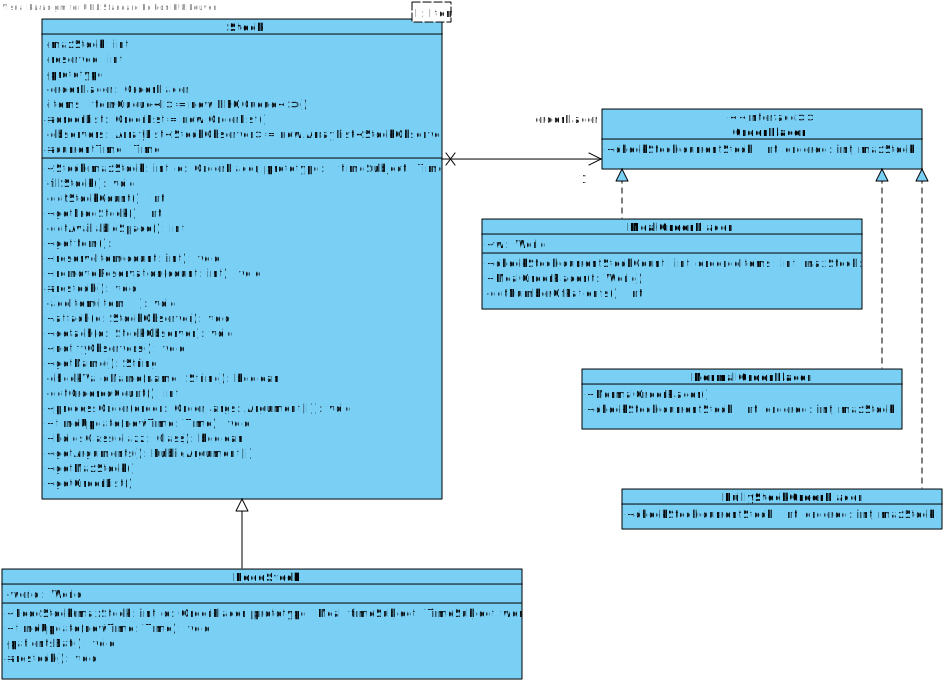
\includegraphics[width=\textwidth]{Pictures/StockOrder}
\caption{Klasse diagram van het systeem om de Stock te vullen}
\label{fig:StockOrder}
\end{figure}

\subsubsection{Bespreking GRASP en uitbreidbaarheid}
Het voordeel van het gebruiken van het Strategy patroon is dat de Stock onafhankelijk word van het algoritme om te bepalen hoeveel er moet worden bijbesteld. Dit maakt het systeem ook meer uitbreidbaar omdat er nu makkelijk een nieuw soort items kan toegevoegt worden en 1 van de bestaande OrderPlacers kan gebruikt worden. De klasse OrderPlacer heeft ook een zeer hoge cohesie aangezien deze enkel verantwoordelijk is voor het bepalen van de te bestellen hoeveelheid. In onze oplossing voor voedsel is ons ontwerp niet zo heel goed. Een beter ontwerp zou zijn om volgens het GRASP pattern pure fabrication een klasse te maken die als verantwoordelijkheid heeft om het bestellen en verbruiken van voedsel items te leiden op de juiste tijdstippen. Hierdoor is er geen speciale subklasse van Stock nodig. Ook voor de cohesie is dit goed aangezien de klasse Stock dan enkel nog verantwoordelijk is voor het management van de voorraad en deze nieuwe klasse dan de verantwoordelijkheid voor het verbruiken en bijbestellen heeft.

\subsection{List orders}
De UI geeft alle stocknames weer door deze via de worldcontroller aan de warehouse te vragen. Na de keuze van de gebruiker voor \'e\'en bepaalde stock, zal de aangemaakte WareHouseController de orders opvragen aan de stock in de warehouse. Vervolgens filtert hij de niet-gearriveerde orders eruit en ten slotte neemt hij de 20 laatste van de lijst, zoals gevraagd in de usecase.

\section{Public API}

We hebben ervoor gekozen om het pakket Hospital en dus ook zijn sub pakketten in de capsule SystemAPI te zetten. Aangezien de gebruikersinterface klassen buiten dit pakket in het pakket HospitalUI zitten, kan er aan de hand van de tool gecheckt worden of er geen methodes worden gebruikt die geen onderdeel zijn van onze api. Het grootste gedeelte van onze API bevind zich in het pakket Hospital.Controllers verder bevat ook het pakket Hospital.Argument een deel van de API. Er zijn nog 2 klassen buiten deze twee pakketten die een stuk van de API bevatten, namelijk de klasse DiagnosisInfo en LoginInfo. Deze twee klassen zijn gemaakt om informatie door te geven aan de API. Aangezien deze tool de encapsulatie van de capsule checkt kunnen we er van uit gaan dat mits een goede API te kiezen, we een goede afscherming hebben van het domein. Onze API bestaat voornamelijk uit de controllers. In deze controllers wordt alle invoer grondig gecontroleerd op fouten. Dit zorgt voor een goede afscherming van de gebruikersinterface.

\section{Conclusie}
Wat we nu gezien hebben is systeem dat zeer eenvoudig uitbreidbaar is: voor elk type object in het systeem, zij het nu personeel, machines, behandelingen of iets anders, kan men eenvoudig een nieuw soort object aanmaken door een subklasse aan te maken van de juiste hoofdklasse. Enkele functie-implementaties en overrides later is het nieuwe object toegevoegd aan het systeem.
Deze flexibiliteit komt echter ook met een kost: men moet controleren of men wel met het juiste soort object aan het werken is, en sommige functie-aanroepen zijn er iets gecompliceerder door geworden, zoals eerst het aantal en type argumenten moeten opvragen om mee te geven aan een Factory object. De voordelen wegen echter veel zwaarder door dan deze nadelen.

Ons systeem is ook zeer defensief: ongeveer alles wat fout kan lopen wordt tegengehouden door een exception. De verscheidenheid in deze exceptions zorgt ervoor dat men aan de hand van het type exception bijna direct weet wat er misgelopen is, vaak zelfs zonder de documentatie te moeten raadplegen.
Voor de laatste iteratie hebben we ervoor gekozen sommige exceptions wat algemener te maken of samen te brengen onder een algemenere parent-exception. Hierdoor moeten er in de code minder verschillende exceptions afgehandeld worden en wordt het systeem eenvoudiger om mee te werken.


\section{Appendices}
%\subsection{Mogelijke uitbreidingen} wordt eigelijk al besproken in de conclusie
\subsection{De user interface \label{sec:ui}}
De UserInterface bestaat uit \'e\'en MainUI, \'e\'en rolUI per rol die kan inloggen en \'e\'en usecaseUI per usecase.
In de MainUI krijg je de optie om in te loggen en na het inloggen zal de UI van de juiste rol (bvb. Doctor, WareHouseManager, ...) gestart worden.
In de rolUI krijg je alle usecaseopties die voor die bepaalde rol gelden en wordt er gefiltert op precondities. Zo zal de DocterUI enkel de optie ClosePatientFile aanbieden, als de doctor van de huidige doctorcontroller een patient file open heeft.
In de usecaseUI wordt heel de usecase doorlopen: lijsten worden getoond, er worden opties aangeboden, invoer gevraagd, ...

\subsection{Testverslag}
\subsubsection{Teststrategie}
Het testen is voortgezet geweest zoals in het vorige semester. Er zijn een aantal scenarios opgesteld die de volledige API testen, in andere tests wordt een deel van de API getest. Het schedulen van afspraken is uitvoerig getest geweest. Alle constraints worden getest op uitzonderingsgevallen. Ook de AppointmentConstraintSolver werd getest.

Dit is zoals voorzien in ons testverslag van vorig semester.

\subsubsection{Eclemma-verslag} %het verslag zelf moet hier nog bijgevoegd worden
Eclemma rapporteert in tegenstelling tot iteratie 2 een redelijke coverage van 70\%. Dit komt omdat de code van de UI afgescheiden is geweest naar een apart project. Ook zijn ongebruikte klassen verwijderd of in gebruik genomen, met de nodige testen. De minst geteste klasses zijn nog steeds de exceptions.

Echter de beste aanduiding van de kwaliteit van onze testsuite is het feit dat doorheen het implementeren van de software we gebruik hebben kunnen maken van onze tests om fouten in het systeem te kunnen opsporen. Deze ervaring van nut uit de tests gehaald te kunnen hebben zonder onzekerheid of het systeem nu wel \'echt\' werkt is waarschijnlijk ook de beste indicator voor testsuite-kwaliteit.

\begin{figure}[h]
\centering
\caption{Eclemma code coverage verslag voor de testsuite}
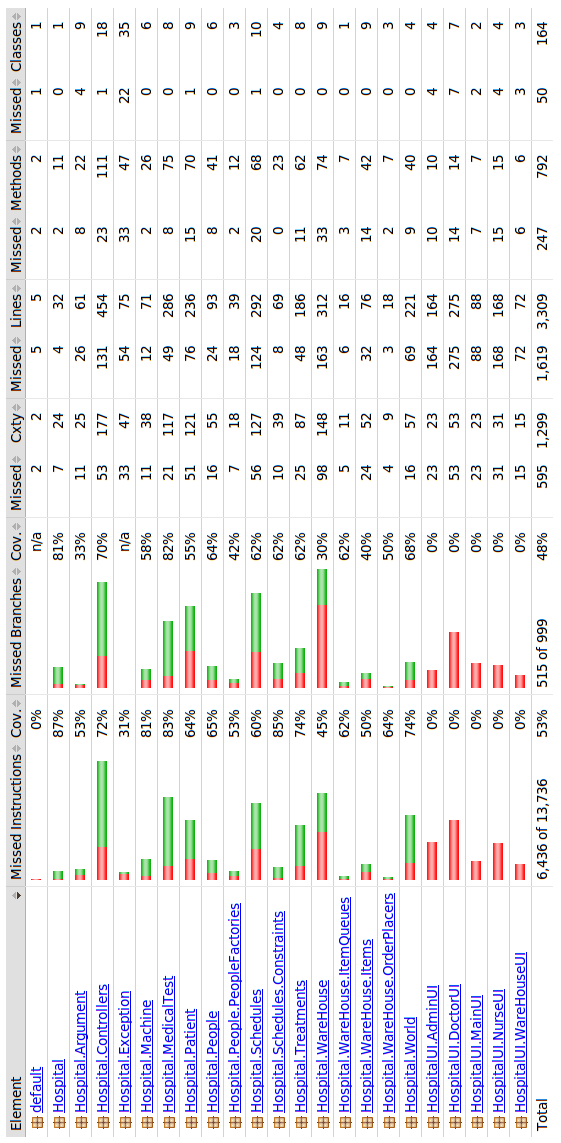
\includegraphics[height=\textheight]{Pictures/Eclemma}
\label{fig:eclemma}
\end{figure}
\subsection{Werkverdeling} %dit moet gewoon een tabel worden zeker? (met de uren en onderwerpen van het werk van iedereen)
\begin{center}
\begin{tabular}{| r || c | l |}
\hline
De Bie Tom & 37u & register patient, API, Scenariotest, kleine aanpassingen \\
\hline
De Coninck Jeroen & 46u & Refactoring, Campusssen, Verslag \\
\hline
Lapauw Ruben & \~ 62u & Scheduling, AddEquipment \& AddStaffMembers \\
	     &		 & Warehouse, Verslag \\
\hline
Van Gool Jeroen & 40u & Diagnoses, MedicalTest \& Verslag \\ 
~ & ~ & Verslag \\
\hline
\end{tabular}
\end{center}
\newpage
\subsection{Volledig klassendiagram \label{sec:classdiagram}}
druk dit apart af gespreid over 2 paginas en voeg in in plaats van dit blad
\newpage
\end{document}
